\section{Resultados preliminares}
Se presentan las verificaciones de conservación y las comparaciones entre integradores para evaluar el modelo numérico (objetivos 1 y 2), seguidas del análisis de separación de escalas y de dos escenarios de acoplamiento informativo (objetivos 3 y 4). Además de variar $\varepsilon$, se realizaron barridos independientes de $b_1$, $b_2$, $K$ y $\beta$ para estudiar la sensibilidad de la infección (objetivo 3).
\subsection{Conservación y comparación de integradores}
En los dos estados iniciales y con $h=0.1$, todas las simulaciones terminaron sin poblaciones negativas. Para la condición alternativa, la tabla \ref{tab:errores} sintetiza los errores frente a \texttt{ode45}, las evaluaciones de función y la conservación. En la configuración mostrada, RK4 obtuvo el menor error, mientras RKF45 consiguió una aproximación del mismo orden decimal con menos evaluaciones de $\mathbf f$. No se infiere de ello una superioridad universal ni una comparación con exactitud equivalente: RKF45 adaptó automáticamente la malla, a diferencia de los otros métodos.

\begin{table}[t]
\centering\footnotesize
\caption{Precisión en $T=100$, $\varepsilon=0.01$, condición alternativa y paso fijo o inicial $h=0.1$.}
\label{tab:errores}
\begin{tabular}{lrrr}
\toprule Método & Error máximo & Eval. $\mathbf f$ & Error cons. \\ \midrule
Euler explícito & $1.2883\cdot10^{-3}$ & 1000 & $1.11\cdot10^{-15}$ \\
RK4 & $7.3493\cdot10^{-10}$ & 4000 & $8.88\cdot10^{-16}$ \\
RKF45 & $1.1960\cdot10^{-9}$ & 702 & $2.22\cdot10^{-16}$ \\
Euler atrás & $1.2392\cdot10^{-3}$ & 4150 & $7.15\cdot10^{-11}$ \\
\bottomrule
\end{tabular}
\par{\scriptsize\textit{Nota.} Eval. $\mathbf f$: evaluaciones; Error cons.: desviación máxima.\par}
\end{table}

La reducción del error al dividir $h$ entre dos fue aproximadamente proporcional a $h$ para ambos métodos de Euler. En el escenario original RK4 disminuyó de $1.7938\cdot10^{-8}$ ($h=0.4$) a $1.1081\cdot10^{-9}$ ($h=0.2$), con razón de $16.19$ y orden observado próximo a cuatro. Los resultados a pasos aún menores se interpretaron con cautela por la presencia de errores próximos a la precisión de la referencia. La figura \ref{fig:convergencia} permite comparar órdenes en escala logarítmica.
\begin{figure}[t]
\centering\figpng{fig01_convergencia_alternativa.png}
\caption{Errores de Euler y RK4 frente a referencia según el paso fijo. Programa MATLAB 05; ambos ejes se muestran en escala logarítmica.}
\label{fig:convergencia}
\end{figure}

La adaptación automática se comprobó adicionalmente mediante la secuencia de pasos aceptados de RKF45, cuyo tamaño respondió a los cambios de la dinámica informativa. Esta figura muestra el mecanismo computacional que permitió reducir el número de evaluaciones; no constituye una comparación de estabilidad absoluta.

\begin{figure}[t]
\centering\figpng{fig05_paso_adaptativo_rkf45.png}
\caption{Evolución del paso aceptado por RKF45 para la condición inicial alternativa. Programa MATLAB 03 (panel ``Adaptación del paso'').}
\label{fig:rkf45_pasos}
\end{figure}

\subsection{Rigidez, estabilidad y costo computacional}
Al disminuir $\varepsilon$ de $0.1$ a $0.01$ y $0.001$, el indicador espectral local aumentó de $12.8959$ a $159.107$ y $1633.49$. Al fijar $\tau_f=1$, esta comparación cubrió horizontes rápidos de 10, 100 y 1000, respectivamente. El crecimiento de la razón es consistente con la separación de escalas, sin ser una prueba independiente de rigidez global.

\begin{table}[t]
\centering\footnotesize
\caption{Resultado con paso nominal $h=4$ según la separación temporal.}
\label{tab:rigidez}
\begin{tabular}{cclll}
\toprule $\varepsilon$ & SR & Euler exp. & RK4 & Euler atrás \\ \midrule
$0.1$ & 12.90 & Válido & Válido & Válido \\
$0.01$ & 159.11 & No admisible$^{\dagger}$ & Inadmisible & Válido* \\
$0.001$ & 1633.49 & Inadmisible & Inadmisible & Válido* \\
\bottomrule

\end{tabular}
\par{\scriptsize\textit{Nota.} SR: razón espectral; $^{\dagger}$inadmisible por restricciones; *válido tras reducir $h$.\par}
\end{table}

Para $\varepsilon=0.01$ y $h=4$, Euler explícito presentó violación de restricciones y RK4 quedó clasificado como inadmisible. La implementación implícita finalizó con error máximo $0.03116$ respecto a \texttt{ode15s}, pero necesitó 39 pasos aceptados y 18 rechazados. Para $\varepsilon=0.001$ y $h=4$, Euler hacia atrás registró 365 pasos aceptados y 153 rechazados, con error aproximado $0.0305$. La diferencia revela una ventaja de robustez del procedimiento implementado en esos experimentos, a costa de resolver múltiples sistemas internos y reducir pasos. No se atribuye ese resultado únicamente a la estabilidad absoluta teórica del integrador.
\begin{figure*}[!t]
\centering
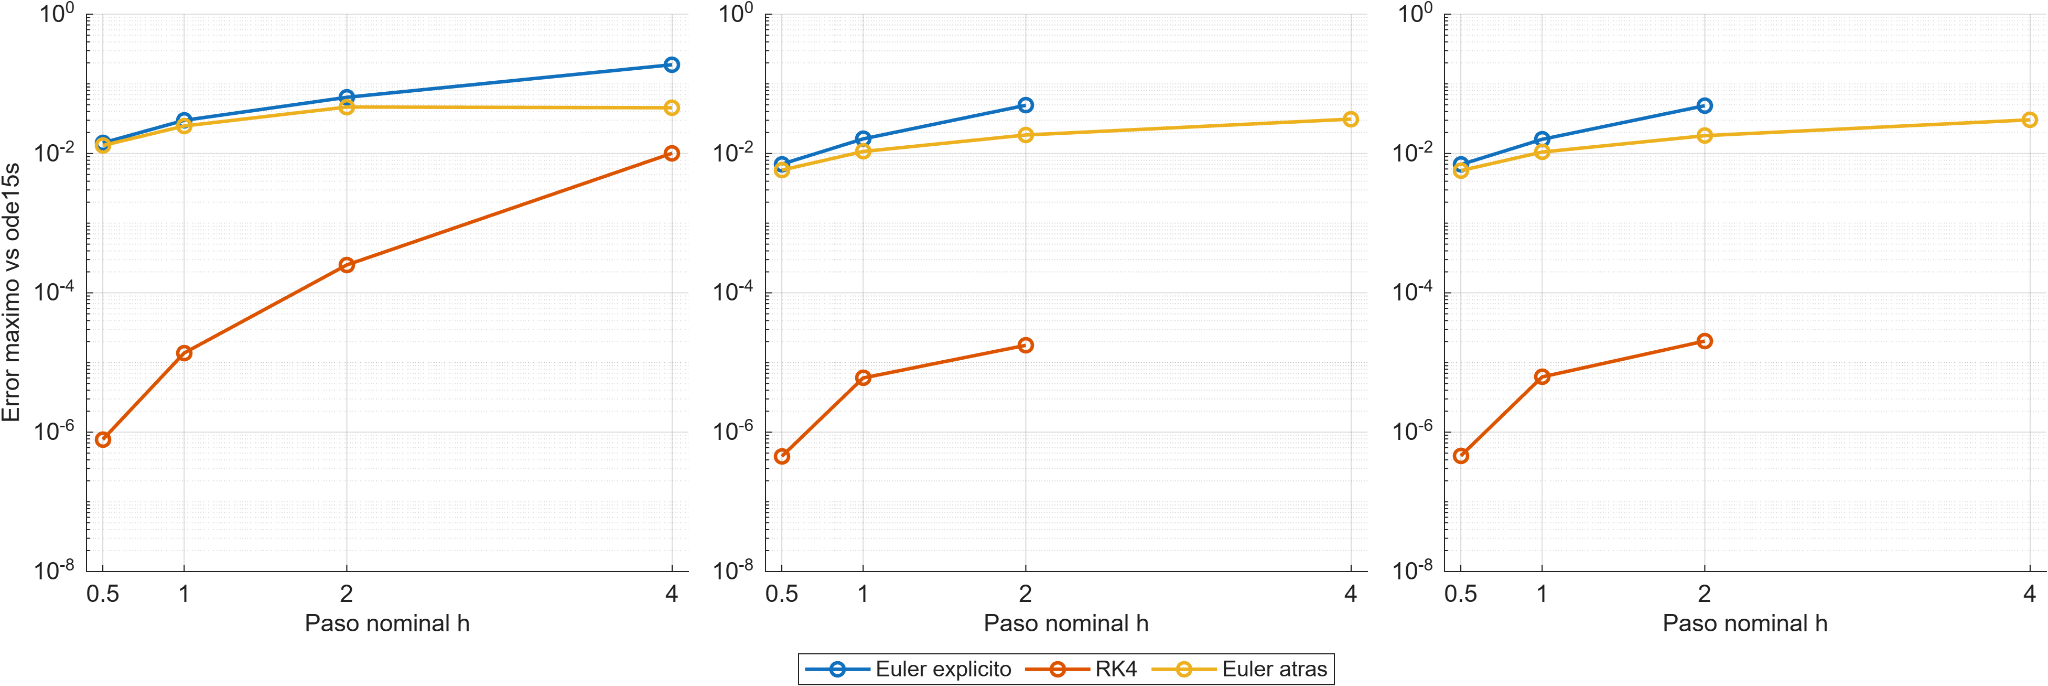
\includegraphics[width=0.91\textwidth]{imagenes/fig02_rigidez_estabilidad.png}
\caption{Error máximo frente a \texttt{ode15s} según el paso nominal para $\varepsilon=0.1$, $0.01$ y $0.001$ (paneles de izquierda a derecha). El eje vertical es logarítmico para distinguir los errores de RK4. Solo aparecen los casos admisibles.}
\label{fig:rigidez}
\end{figure*}

\subsection{Variación de parámetros}
Se varió un parámetro por ejecución, manteniendo fijos los restantes valores del conjunto exploratorio, con la condición inicial alternativa. La tabla~\ref{tab:parametricos} resume el intervalo de fracciones infectadas finales observado en el CSV exportado por el experimento 08. Todos los casos registrados finalizaron con estado \texttt{OK} y error máximo de conservación menor que $2.5\cdot10^{-15}$. Estos resultados cuantifican sensibilidad local al diseño experimental; no constituyen una calibración epidemiológica ni garantizan tendencias universales.
\begin{table}[!tbp]
\centering\footnotesize
\caption{Variación uniparamétrica: fracción infectada final en los extremos del barrido.}
\label{tab:parametricos}
\begin{tabular}{lcccc}
\toprule
Parámetro & Valor bajo & $I_f$ & Valor alto & $I_f$ \\
\midrule
$b_1$ & 0.5 & 0.3222 & 2.0 & 0.4429 \\
$b_2$ & 0.5 & 0.3892 & 2.0 & 0.2405 \\
$K$ & 0 & 0.3892 & 0.9 & 0.3222 \\
$\beta$ & 2 & 0.0206 & 8 & 0.3792 \\
\bottomrule
\end{tabular}
\par{\scriptsize\textit{Nota.} $I_f$: fracción infectada final; demás parámetros fijos.\par}
\end{table}

\begin{figure*}[!b]
\centering
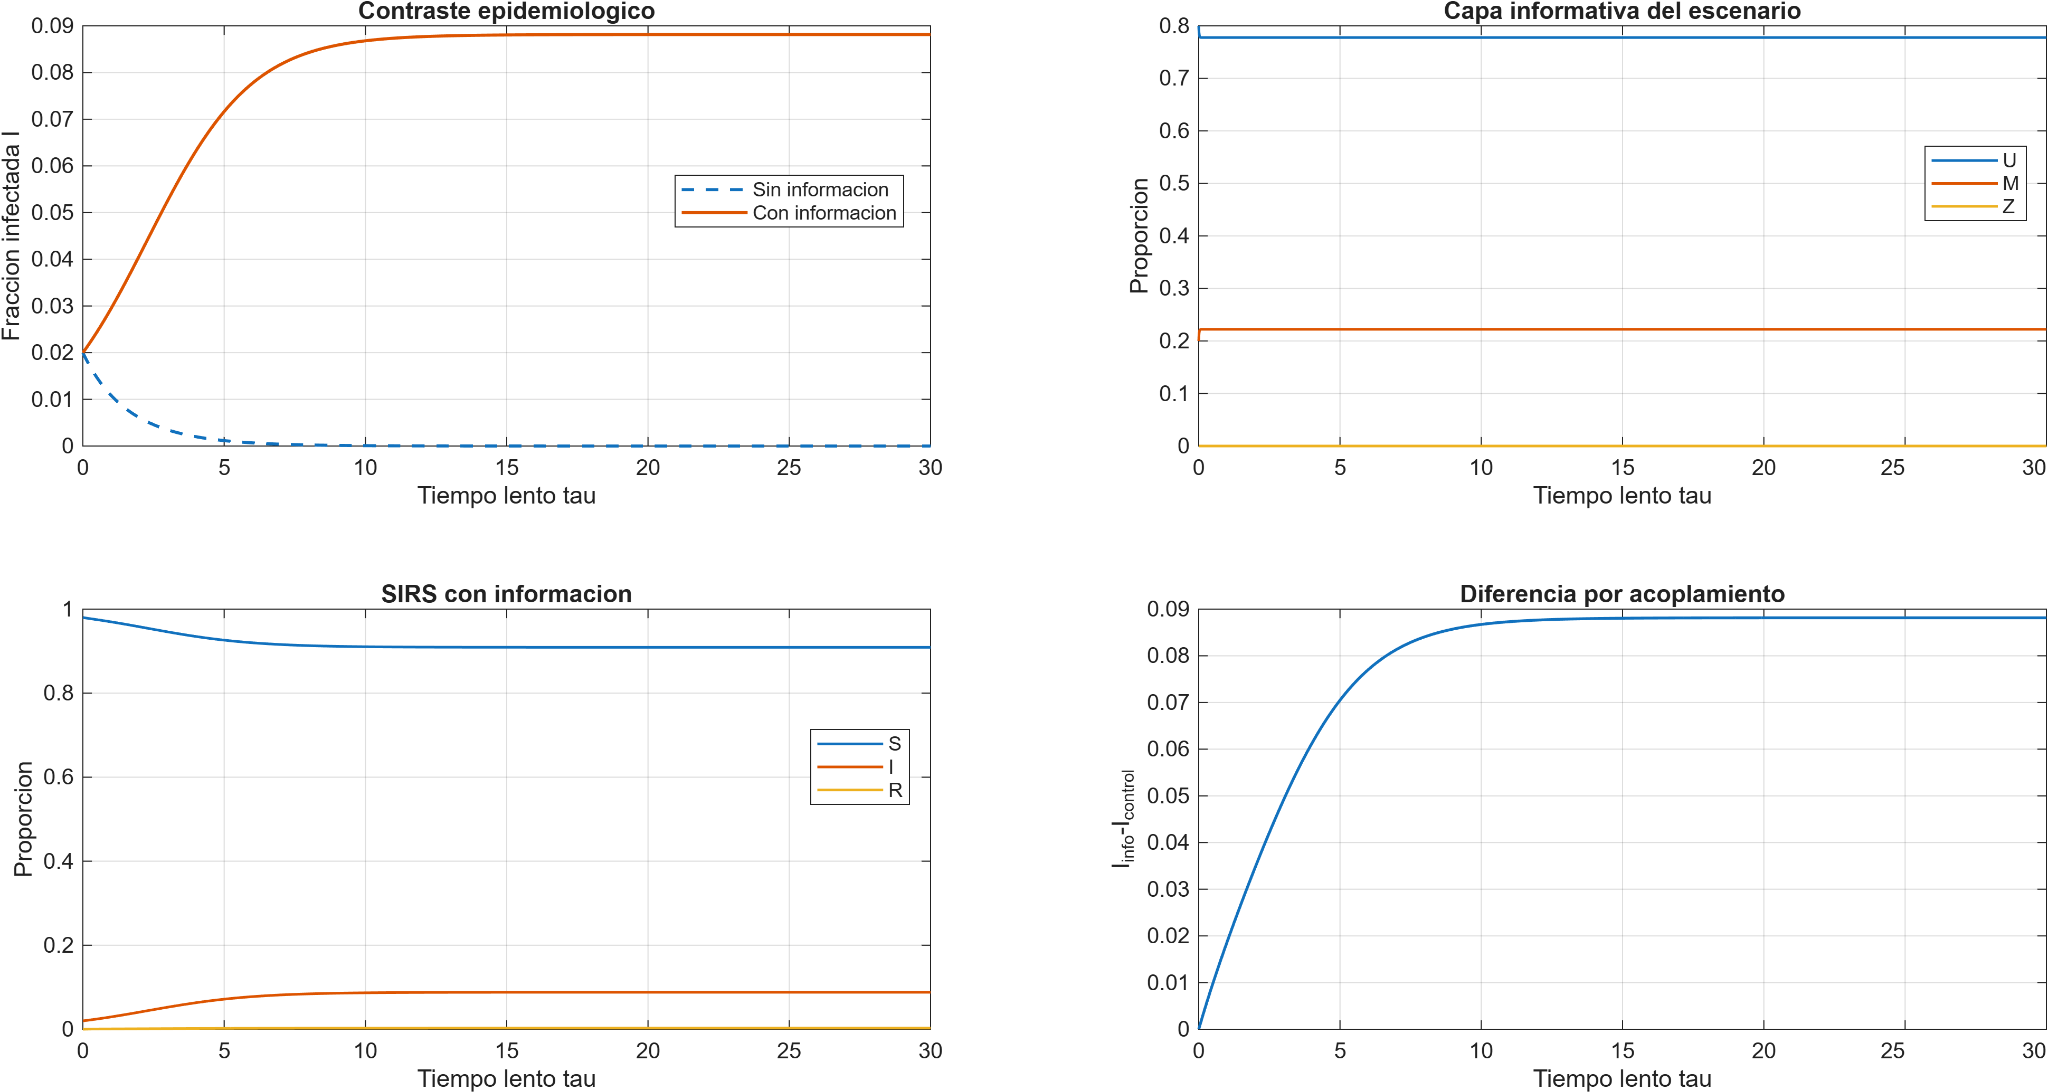
\includegraphics[width=0.72\textwidth]{imagenes/fig03_escenario_desinformacion.png}
\caption{Dinámica epidemiológica con desinformación y control sin difusión informativa. Programa MATLAB 07.}
\label{fig:desinformacion}
\end{figure*}

\subsection{Desinformación y escepticismo}
Se contrastó el efecto del acoplamiento social con un control informativo constante para dos conjuntos de parámetros. La tabla \ref{tab:epidemia} presenta las fracciones infectadas finales en tiempo lento $\tau=30$. En el escenario I, con desinformación, $I$ terminó alrededor de $0.08814$, frente a $1.65\cdot10^{-9}$ en el control. En el escenario II, con escepticismo, terminó en $1.51\cdot10^{-9}$, mientras el control finalizó aproximadamente en $0.08813$.

\begin{table}[t]
\centering\footnotesize
\caption{Fracción infectada al final de los escenarios epidemiológicos ($\tau=30$).}
\label{tab:epidemia}
\begin{tabular}{lrr}
\toprule Escenario & Control & Con acoplamiento \\ \midrule
I: desinformación & $1.6453\cdot10^{-9}$ & $0.08814414$ \\
II: escepticismo & $0.08812925$ & $1.5130\cdot10^{-9}$ \\
\bottomrule
\end{tabular}
\par{\scriptsize\textit{Nota.} Control: sin información; acoplamiento: con información.\par}
\end{table}

En las dos trayectorias acopladas, el error máximo de RK4 respecto a \texttt{ode15s} fue $2.82\cdot10^{-8}$ y $5.47\cdot10^{-8}$, respectivamente. Los errores de conservación estuvieron alrededor de $10^{-15}$ y las componentes permanecieron no negativas. Los controles y las curvas informativas se ilustran en las figuras \ref{fig:desinformacion} y \ref{fig:escepticismo}; representan únicamente los horizontes e hipótesis considerados.



En conjunto, el contraste de integradores mostró diferencias importantes en precisión y en admisibilidad a pasos grandes; al disminuir $\varepsilon$ creció el indicador espectral inicial y se requirió mayor atención a la estabilidad. Los dos escenarios de acoplamiento produjeron respuestas epidémicas opuestas dentro del horizonte simulado, sin que ello constituya una demostración de su comportamiento asintótico. El barrido de parámetros mostró diferencias apreciables en la infección final, sin violar la conservación poblacional en los casos registrados.

\begin{figure*}[!t]
\centering
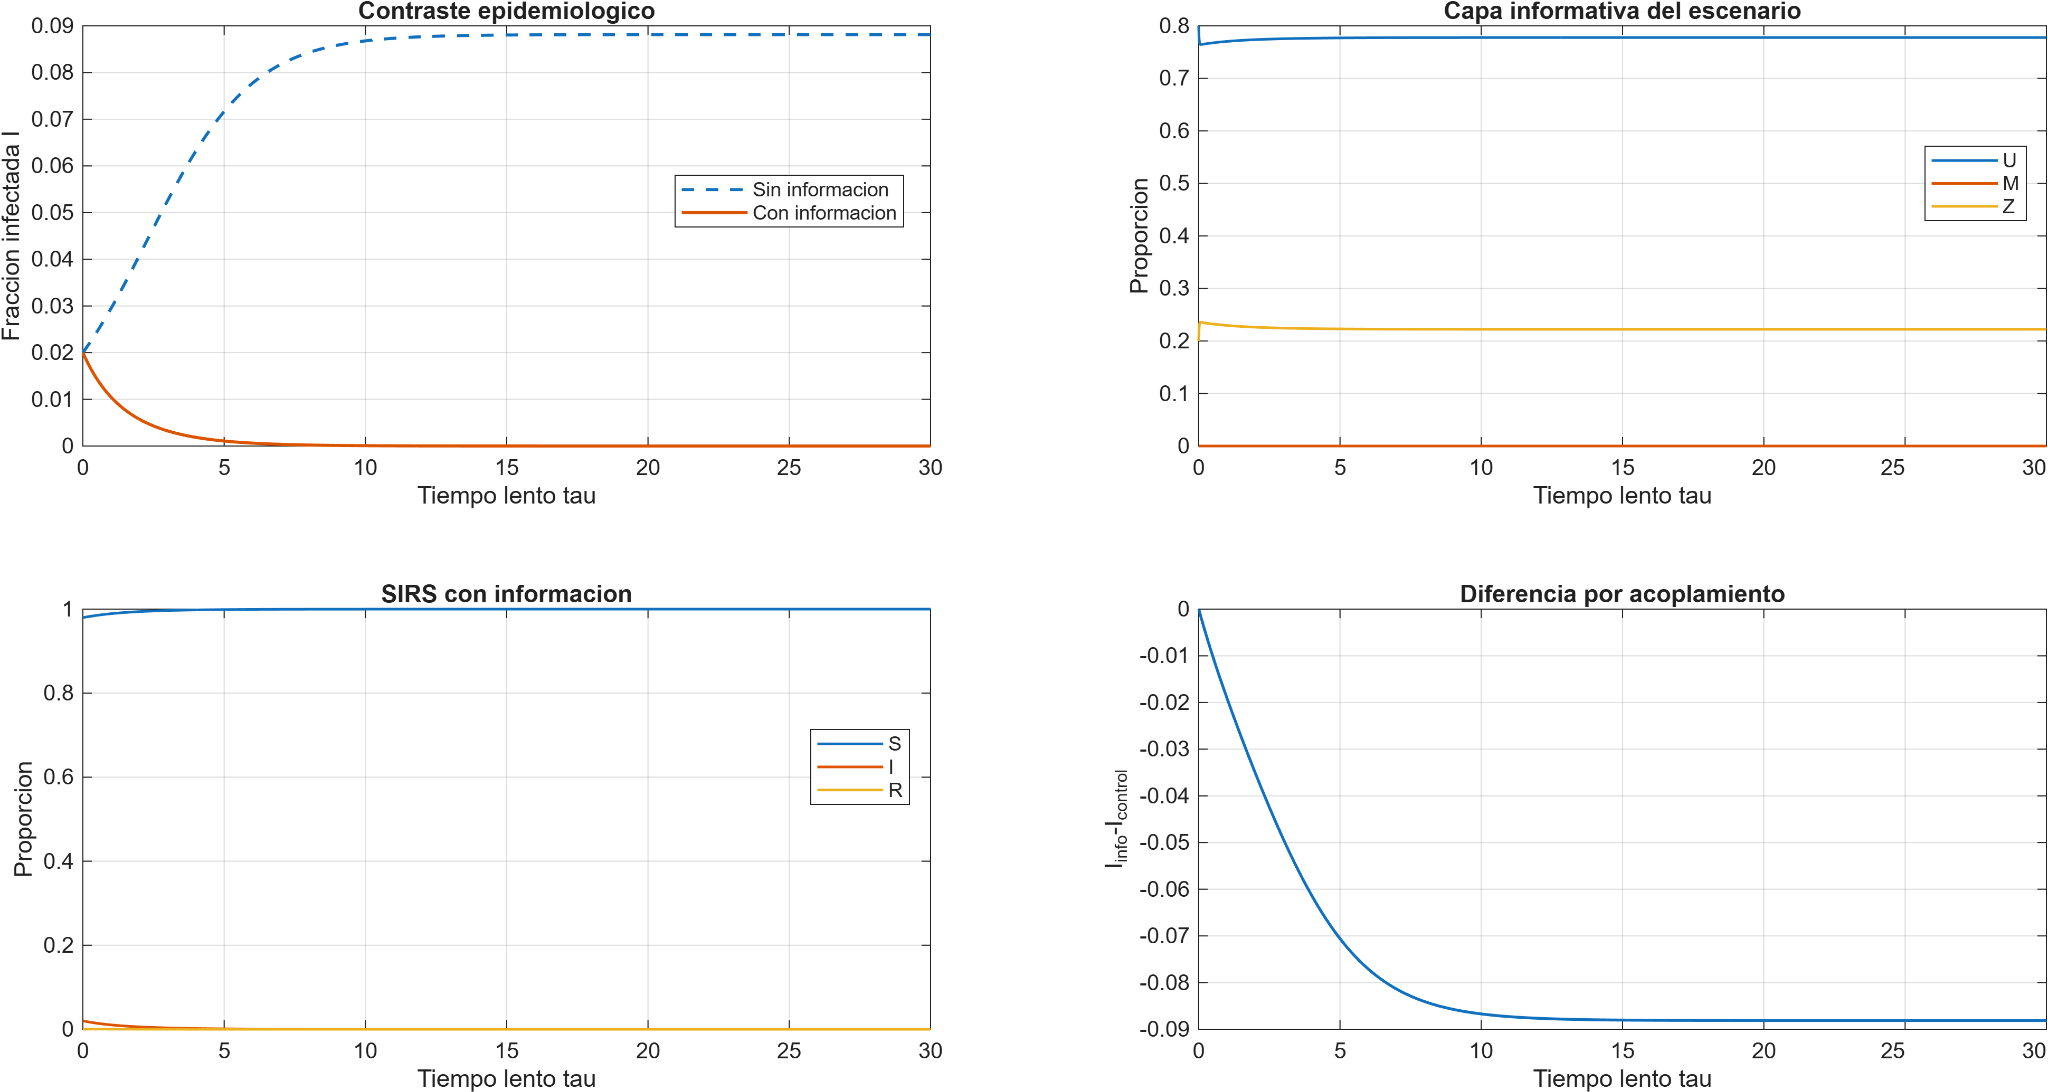
\includegraphics[width=0.72\textwidth]{imagenes/fig04_escenario_escepticismo.png}
\caption{Dinámica epidemiológica con escepticismo y control sin difusión informativa. Programa MATLAB 07.}
\label{fig:escepticismo}
\end{figure*}
